% Animated derivation slides for RNN, Autoencoder, LSTM, CNN-AE, VAE
\documentclass[11pt]{beamer}
\usetheme{Madrid}
\usecolortheme{seagull}
\usefonttheme{professionalfonts}

\usepackage{amsmath,amssymb}
\usepackage{tikz}
\usepackage{graphicx}

% TikZ styles (no color)
\tikzset{
  node/.style={draw, circle, minimum size=10mm},
  cell/.style={draw, rectangle, minimum width=16mm, minimum height=12mm},
  layer/.style={draw, rectangle, minimum width=22mm, minimum height=12mm},
  block/.style={draw, rectangle, minimum width=20mm, minimum height=12mm}
}

\title{Derivations}
\author{RNNs and AEs}
\date{\today}

\begin{document}
\begin{frame}\titlepage\end{frame}

% -------------------------
% RNN: forward equations + BPTT
% -------------------------
\section{RNN: Forward pass and BPTT}
\begin{frame}[<+->]{Vanilla RNN: forward equations}
\begin{itemize}
  \item[$\bullet$] Hidden state update:
  \[
    h_t = \phi(W_{xh} x_t + W_{hh} h_{t-1} + b_h)
  \]
  \item[$\bullet$] Output:
  \[
    y_t = W_{hy} h_t + b_y
  \]
  \item[$\bullet$] Where $\phi$ is e.g. $\tanh$ or ReLU.
\end{itemize}
\end{frame}

\begin{frame}[<+->]{Unroll in time (visual)}
\centering
\begin{tikzpicture}[>=stealth, node distance=1.9cm]
  \node[node] (x1) {$x_1$};
  \node[cell, above=1.5cm of x1] (h1) {$h_1$};
  \node[node, above=1.5cm of h1] (y1) {$y_1$};

  \node[node, right=3cm of x1] (x2) {$x_2$};
  \node[cell, above=1.5cm of x2] (h2) {$h_2$};
  \node[node, above=1.5cm of h2] (y2) {$y_2$};

  \node[node, right=3cm of x2] (x3) {$x_3$};
  \node[cell, above=1.5cm of x3] (h3) {$h_3$};
  \node[node, above=1.5cm of h3] (y3) {$y_3$};

  \draw[->] (x1) -- node[right] {$W_{xh}$} (h1);
  \draw[->] (x2) -- node[right] {$W_{xh}$} (h2);
  \draw[->] (x3) -- node[right] {$W_{xh}$} (h3);

  \draw[->] (h1) -- node[above] {$W_{hh}$} (h2);
  \draw[->] (h2) -- node[above] {$W_{hh}$} (h3);

  \draw[->] (h1) -- node[right] {$W_{hy}$} (y1);
  \draw[->] (h2) -- node[right] {$W_{hy}$} (y2);
  \draw[->] (h3) -- node[right] {$W_{hy}$} (y3);
\end{tikzpicture}
\end{frame}

\begin{frame}[<+->]{Backpropagation Through Time (BPTT) — derivation}
\begin{block}{Loss over sequence}
  \[
    \mathcal{L} = \sum_{t=1}^T \ell(y_t, \hat y_t)
  \]
\end{block}

\visible<2->{We want $\dfrac{\partial \mathcal{L}}{\partial W_{hh}}$. Use chain rule across time:}
\[
\frac{\partial \mathcal{L}}{\partial W_{hh}}
= \sum_{t=1}^T \frac{\partial \mathcal{L}}{\partial h_t} \frac{\partial h_t}{\partial W_{hh}}.
\]

\visible<3->{Compute recursive gradient for hidden states. Define $\delta_t \equiv \frac{\partial \mathcal{L}}{\partial h_t}$. Then}
\[
\delta_t = \frac{\partial \ell_t}{\partial h_t} + \left(\frac{\partial h_{t+1}}{\partial h_t}\right)^\top \delta_{t+1}.
\]

\visible<4->{Since $h_{t+1} = \phi(W_{xh}x_{t+1} + W_{hh}h_t + b)$,}
\[
\frac{\partial h_{t+1}}{\partial h_t} = \operatorname{diag}\big(\phi'(a_{t+1})\big) W_{hh},
\]
with $a_{t+1}=W_{xh}x_{t+1}+W_{hh}h_t+b$.

\visible<5->{Hence the recurrence}
\[
\boxed{\ \delta_t = \nabla_{h_t}\ell_t + W_{hh}^\top \operatorname{diag}\big(\phi'(a_{t+1})\big) \delta_{t+1}\ }
\]
and the parameter gradient:
\[
\frac{\partial \mathcal{L}}{\partial W_{hh}} = \sum_{t=1}^T \delta_t \, h_{t-1}^\top .
\]
\end{frame}

\begin{frame}[<+->]{Vanishing / Exploding gradients (intuition)}
\begin{itemize}
  \item Expand recurrence: $\delta_t$ involves products of $\big(W_{hh}^\top \operatorname{diag}(\phi')\big)^{k}$.
  \item If spectral radius $\rho(W_{hh})<1$ (and $\|\phi'\|$ bounded) gradients decay exponentially $\to$ \textbf{vanishing}.
  \item If $\rho(W_{hh})>1$ gradients grow exponentially $\to$ \textbf{exploding}.
  \item Remedies: gradient clipping, orthogonal init, truncated BPTT, gated cells (LSTM/GRU).
\end{itemize}
\end{frame}

% -------------------------
% Deep Autoencoder: derivations (linear -> PCA) and animated slides
% -------------------------
\section{Deep Autoencoder: derivations}
\begin{frame}[<+->]{Autoencoder setup (general)}
\[
z = f_\theta(x),\qquad \hat x = g_\phi(z)
\]
\[
\mathcal{L}(\theta,\phi) = \frac{1}{N}\sum_{i=1}^N \ell\big(x^{(i)}, g_\phi(f_\theta(x^{(i)}))\big).
\]
\visible<2->{Common choice $\ell =$ MSE: $\|x-\hat x\|_2^2$.}
\end{frame}

\begin{frame}[<+->]{Linear autoencoder $\Rightarrow$ PCA (sketch)}
\visible<1->{Assume linear encoder/decoder without biases:}
\[
z = W_e x,\qquad \hat x = W_d z = W_d W_e x.
\]
\visible<2->{Minimize Frobenius norm over data matrix $X\in\mathbb{R}^{d\times N}$:}
\[
\min_{W_d,W_e} \|X - W_d W_e X\|_F^2.
\]
\visible<3->{Set $W = W_d W_e$ with $\operatorname{rank}(W)\le m$. By Eckart--Young: best rank-$m$ approximation to $X$ (in Frobenius norm) is $X_m = U_m \Sigma_m V_m^\top$, the PCA truncation.}
\visible<4->{Thus the column space of optimal $W$ is span of top-$m$ principal components. With orthonormal constraints $W_e = U_m^\top, W_d = U_m$ one recovers PCA projection.}
\end{frame}

\begin{frame}[<+->]{Nonlinear AE: gradient descent}
\[
\frac{\partial \mathcal{L}}{\partial \theta}
= \frac{1}{N}\sum_i \frac{\partial \ell}{\partial \hat x}\frac{\partial \hat x}{\partial z}\frac{\partial z}{\partial \theta},
\]
\visible<2->{autodiff applies backprop through encoder and decoder stacks.}
\end{frame}

% Include deep autoencoder diagram (multi-layer) with overlay reveal
\begin{frame}[<+->]{Deep autoencoder (diagram)}
\centering
\begin{tikzpicture}[>=stealth, node distance=1.8cm]
  \node[layer] (x) {Input $x$};
  \node[layer, right=1.8cm of x] (enc1) {Enc1 \\ $W_1$};
  \node[layer, right=1.4cm of enc1] (enc2) {Enc2 \\ $W_2$};
  \node[layer, right=1.4cm of enc2] (z) {Latent $z$};
  \node[layer, right=1.4cm of z] (dec1) {Dec1 \\ $W_3$};
  \node[layer, right=1.4cm of dec1] (dec2) {Dec2 \\ $W_4$};
  \node[layer, right=1.8cm of dec2] (xhat) {Output $\hat x$};

  \draw[->] (x) -- (enc1);
  \draw[->] (enc1) -- (enc2);
  \draw[->] (enc2) -- (z);
  \draw[->] (z) -- (dec1);
  \draw[->] (dec1) -- (dec2);
  \draw[->] (dec2) -- (xhat);
\end{tikzpicture}
\end{frame}

% -------------------------
% LSTM: equations and derivation incl. gradients sketch
% -------------------------
\section{LSTM: equations and gradients}
\begin{frame}[<+->]{LSTM cell equations (forward)}
\[
\begin{aligned}
i_t &= \sigma(W_i x_t + U_i h_{t-1} + b_i)\\
f_t &= \sigma(W_f x_t + U_f h_{t-1} + b_f)\\
o_t &= \sigma(W_o x_t + U_o h_{t-1} + b_o)\\
\tilde c_t &= \tanh(W_c x_t + U_c h_{t-1} + b_c)\\
c_t &= f_t \odot c_{t-1} + i_t \odot \tilde c_t\\
h_t &= o_t \odot \tanh(c_t).
\end{aligned}
\]
\visible<2->{This structure yields controlled gradient flow via multiplicative gates.}
\end{frame}

\begin{frame}[<+->]{LSTM: gradient flow intuition}
\begin{itemize}
  \item Key term: $c_t = f_t \odot c_{t-1} + \dots$. If $f_t\approx 1$ and $o_t\approx 1$, information (and gradients) flow across many steps with little attenuation.
  \item Gradient w.r.t. $c_{t-1}$:
  \[
    \frac{\partial \mathcal{L}}{\partial c_{t-1}} = \frac{\partial \mathcal{L}}{\partial c_t} \odot f_t + \dots
  \]
  so $f_t$ acts multiplicatively on gradients, allowing the cell to preserve or forget information dynamically.
\end{itemize}
\end{frame}

\begin{frame}[<+->]{LSTM cell diagram (animated reveal)}
\centering
\begin{tikzpicture}[>=stealth, node distance=1.6cm]
  \node[circle, draw] (xt) {$x_t$};
  \node[rectangle, draw, right=1.8cm of xt] (i) {Input gate $i_t$};
  \node[rectangle, draw, above=0.7cm of i] (f) {Forget $f_t$};
  \node[rectangle, draw, below=0.7cm of i] (o) {Output $o_t$};
  \node[rectangle, draw, right=2.3cm of i] (ct) {$c_t$};
  \node[circle, draw, right=1.6cm of ct] (ht) {$h_t$};

  \draw[->] (xt) -- (i);
  \draw[->] (xt) -- (f);
  \draw[->] (xt) -- (o);

  \draw[->] (i) -- (ct);
  \draw[->] (f) -- (ct);
  \draw[->] (ct) -- (ht);
  \draw[->] (o) -- (ht);

  \node[above=0.2cm of ct] {$c_{t-1}$};
  \draw[->] ($(ct)+(-1.8,0.7)$) -- (ct);
\end{tikzpicture}
\end{frame}

% -------------------------
% CNN Autoencoder: small derivation on receptive field, architecture
% -------------------------
\section{CNN Autoencoder}
\begin{frame}[<+->]{CNN-AE: architecture idea}
\begin{itemize}
  \item Encoder: sequence of Conv + nonlinearity + Pool (downsample) $\Rightarrow$ latent.
  \item Decoder: sequence of Upsample (or transpose-conv) + Conv $\Rightarrow$ reconstruction.
\end{itemize}
\end{frame}

\begin{frame}[<+->]{Convolution arithmetic (quick notes)}
\[
\text{output size } = \left\lfloor \frac{H + 2P - K}{S} \right\rfloor + 1,
\]
where $K$ kernel, $S$ stride, $P$ padding. Use transpose-convolution (deconv) to invert downsampling or use upsampling + conv.
\end{frame}

\begin{frame}[<+->]{CNN Autoencoder diagram}
\centering
\begin{tikzpicture}[>=stealth, node distance=1.6cm]
  \node[block] (x) {Input Image};
  \node[block, right=1.8cm of x] (conv1) {Conv};
  \node[block, right=1.6cm of conv1] (pool1) {Pool};
  \node[block, right=1.6cm of pool1] (conv2) {Conv};
  \node[block, right=1.6cm of conv2] (pool2) {Pool};
  \node[block, right=2cm of pool2] (z) {Latent};
  \node[block, right=2cm of z] (up1) {Upsample};
  \node[block, right=1.6cm of up1] (deconv1) {Deconv};
  \node[block, right=1.6cm of deconv1] (xhat) {Reconstruction};

  \draw[->] (x) -- (conv1) -- (pool1) -- (conv2) -- (pool2) -- (z);
  \draw[->] (z) -- (up1) -- (deconv1) -- (xhat);
\end{tikzpicture}
\end{frame}

% -------------------------
% VAE: ELBO derivation and reparameterization
% -------------------------
\section{Variational Autoencoder (VAE)}
\begin{frame}[<+->]{VAE: goal and generative model}
Assume generative model $p_\theta(x,z)=p_\theta(x|z)p(z)$ with prior $p(z)=\mathcal{N}(0,I)$. The marginal likelihood is:
\[
p_\theta(x)=\int p_\theta(x|z)p(z)\,dz,
\]
intractable in general.
\end{frame}

\begin{frame}[<+->]{ELBO derivation (stepwise)}
\begin{align*}
\log p_\theta(x)
&= \log \int p_\theta(x|z)p(z)\,dz \\
&= \log \int q_\phi(z|x)\frac{p_\theta(x|z)p(z)}{q_\phi(z|x)}\,dz \\
&\ge \int q_\phi(z|x) \log\frac{p_\theta(x|z)p(z)}{q_\phi(z|x)} \,dz \quad\text{(Jensen)}\\
&= \mathbb{E}_{q_\phi(z|x)}[\log p_\theta(x|z)] - \mathrm{KL}\big(q_\phi(z|x)\,\|\,p(z)\big) \\
&\equiv \mathcal{L}(\theta,\phi; x) \quad\text{(ELBO)}.
\end{align*}
\visible<2->{Maximizing ELBO $\approx$ maximizing a lower bound on $\log p_\theta(x)$.}
\end{frame}

\begin{frame}[<+->]{Reparameterization trick}
\[
z \sim q_\phi(z|x)=\mathcal{N}(\mu_\phi(x),\Sigma_\phi(x))
\]
Instead sample $\epsilon\sim\mathcal{N}(0,I)$ and set
\[
z = \mu_\phi(x) + L_\phi(x)\,\epsilon,
\]
where $L_\phi$ is e.g. lower-triangular matrix s.t. $L_\phi L_\phi^\top = \Sigma_\phi$. For diagonal covariances:
\[
z = \mu_\phi(x) + \sigma_\phi(x)\odot \epsilon.
\]
This makes gradients w.r.t. $\phi$ tractable via backprop.
\end{frame}

\begin{frame}[<+->]{VAE training objective (practical)}
For Gaussian decoder (and diagonal posterior) the ELBO per datapoint:
\[
\mathcal{L}(\theta,\phi;x)
= \mathbb{E}_{q_\phi(z|x)}[\log p_\theta(x|z)] - \tfrac{1}{2}\sum_j\big(1 + \log \sigma_j^2 - \mu_j^2 - \sigma_j^2\big).
\]
Implement with Monte Carlo estimate (often single sample) and backprop through reparameterization.
\end{frame}


\begin{frame}{Variational Autoencoder (VAE)}









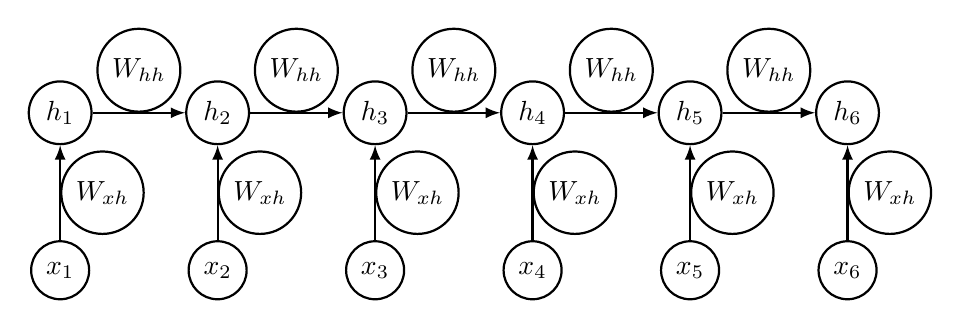
\begin{tikzpicture}[>=latex, thick, every node/.style={draw,circle,fill=white,minimum size=6mm}]
  % Input and hidden state nodes (t=1..6)
  \foreach \i in {0,...,5}{
    \pgfmathtruncatemacro{\num}{\i+1}
    \node (x\num) at ({2*\i},0) {$x_{\num}$};
    \node (h\num) at ({2*\i},2) {$h_{\num}$};
  }
  % Arrows: input-to-hidden (W_{xh})
  \foreach \i in {1,...,6}{
    \draw[->] (x\i.north) -- node[midway,right] {$W_{xh}$} (h\i.south);
  }
  % Arrows: hidden-to-hidden (W_{hh})
  \foreach \i/\j in {1/2,2/3,3/4,4/5,5/6}{
    \draw[->] (h\i.east) -- node[midway,above] {$W_{hh}$} (h\j.west);
  }
\end{tikzpicture}

\end{frame}
\end{document}


